\chapter{Практические задания}

\section{Задача 1}

Представить следующие списки в виде списочных ячеек:

\begin{itemize}
	\item \texttt{'(open close halph)}
	
	\begin{figure}[ht]
		\centering
		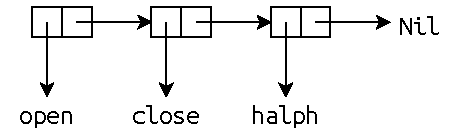
\includegraphics[scale=1]{img/1-1}
	\end{figure}
	
	\item \texttt{'((open1) (close2) (halph3))}
	
	\begin{figure}[ht]
		\centering
		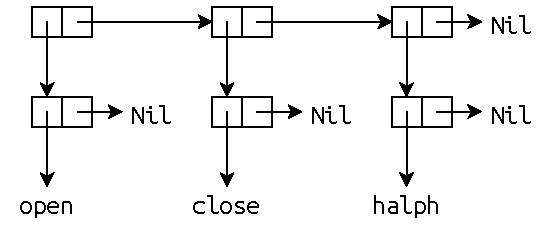
\includegraphics[scale=1]{img/1-2}
	\end{figure}
	
	\item \texttt{'((one) for all (and (me (for you))))}
	
	\begin{figure}[ht]
		\centering
		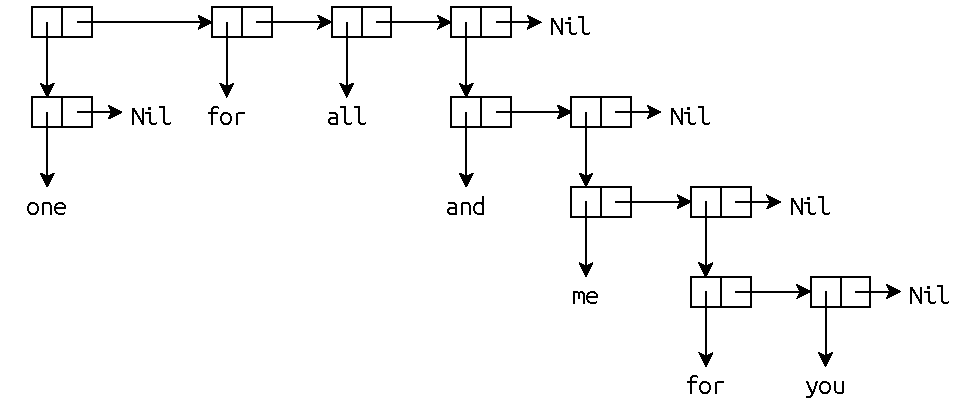
\includegraphics[scale=1]{img/1-3}
	\end{figure}

	\clearpage
	
	\item \texttt{'((TOOL) (call))}
	
	\begin{figure}[ht]
		\centering
		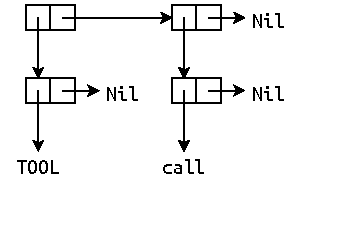
\includegraphics[scale=1.2]{img/1-4}
	\end{figure}
	
	\item \texttt{'((TOOL1) ((call2)) ((sell)))}
	
	\begin{figure}[ht]
		\centering
		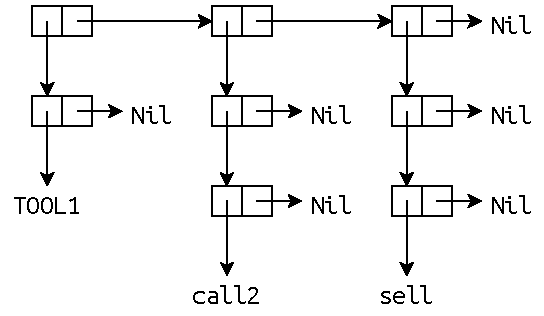
\includegraphics[scale=1]{img/1-5}
	\end{figure}
	
	\item \texttt{'(((TOOL) (call)) ((sell)))}
	
	\begin{figure}[ht]
		\centering
		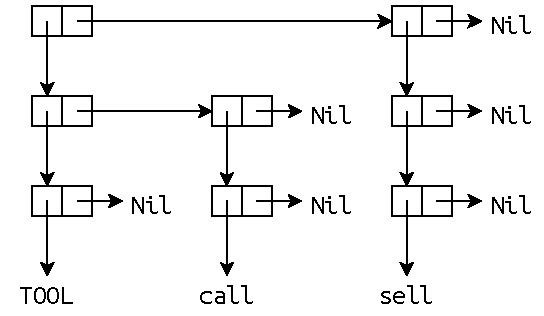
\includegraphics[scale=1]{img/1-6}
	\end{figure}
\end{itemize}

\clearpage

\section{Задача 2}

Используя только функции \texttt{CAR} и \texttt{CDR}, написать выражения, возвращающие:

\begin{enumerate}
	\item второй элемент заданного списка \texttt{x}:
	
	\hspace{2cm} \texttt{(car (cdr x))}
	
	\item третий элемент заданного списка \texttt{x}:

	\hspace{2cm} \texttt{(car (cdr (cdr x)))}
	
	\item четвертый элемент заданного списка \texttt{x}:

	\hspace{2cm} \texttt{(car (cdr (cdr (cdr x))))}
\end{enumerate}

\section{Задача 3}

Каким будет результат вычисления выражений?

\begin{enumerate}[a)]
	\item \texttt{(caadr '((blue cube) (red pyramid)))}
	
	\hspace{2cm} Результат: \texttt{RED}
	
	\item \texttt{(cdar '((abc) (def) (ghi)))}
	
	\hspace{2cm} Результат: \texttt{NIL}
	
	\item \texttt{(cadr '((abc) (def) (ghi)))}
	
	\hspace{2cm} Результат: \texttt{(DEF)}
	
	\item \texttt{(caddr '((abc) (def) (ghi)))}
	
	\hspace{2cm} Результат: \texttt{(GHI)}
\end{enumerate}

\section{Задача 4}

Написать результат вычисления выражений и объяснить, как он получен.

\begin{table}
	\begin{center}
		\begin{tabular}{|l|l|}
			\hline
			\textbf{Выражение} & \textbf{Результат} \\
			\hline
			\texttt{(list 'Fred 'and 'Wilma)} & \texttt{(FRED AND WILMA)} \\
			\hline
			\texttt{(list 'Fred '(and Wilma))} & \texttt{(FRED (AND WILMA))} \\
			\hline
			\texttt{(cons Nil Nil)} & \texttt{(NIL)} \\
			\hline
			\texttt{(cons T Nil)} & \texttt{(T)} \\
			\hline
			\texttt{(cons Nil T)} & \texttt{(Nil . T)} \\
			\hline
			\texttt{(list Nil)} & \texttt{(NIL)} \\
			\hline
			\texttt{(cons '(T) Nil)} & \texttt{((T))} \\
			\hline
			\texttt{(list '(one two) '(free temp))} & \texttt{((ONE TWO) (FREE TEMP))} \\
			\hline
		\end{tabular}
	\end{center}
\end{table}

\clearpage

\begin{table}[ht]
	\begin{center}
		\begin{tabular}{|l|l|}
			\hline
			\textbf{Выражение} & \textbf{Результат} \\
			\hline			
			\texttt{(cons 'Fred '(and Wilma))} & \texttt{(FRED AND WILMA)} \\
			\hline
			\texttt{(cons 'Fred '(Wilma))} & \texttt{(FRED WILMA)} \\
			\hline
			\texttt{(list Nil Nil)} & \texttt{(NIL NIL)} \\
			\hline
			\texttt{(list T Nil)} & \texttt{(T NIL)} \\
			\hline
			\texttt{(list Nil T)} & \texttt{(NIL T)} \\
			\hline
			\texttt{(cons T (list Nil))} & \texttt{(T NIL)} \\
			\hline
			\texttt{(list '(T) Nil)} & \texttt{((T) NIL)} \\
			\hline
			\texttt{(cons '(one two) '(free temp))} & \texttt{((ONE TWO) FREE TEMP)} \\
			\hline
		\end{tabular}
	\end{center}
\end{table}

\section{Задача 5}

Необходимо написать лямбда-выражение и соответствующую функцию. Результат функции представить в виде списковых ячеек.

\begin{itemize}
	\item Написать функцию \texttt{(f ar1 ar2 ar3 ar4)}, возвращающую список \texttt{((ar1 ar2) (ar3 ar4))}:
	
\begin{lstlisting}[language=Lisp]
; lambda-выражение
(lambda (ar1 ar2 ar3 ar4)
	(list (list ar1 ar2) (list ar3 ar4))
)

; именованая функция
(defun f (ar1 ar2 ar3 ar4)
	(list (list ar1 ar2) (list ar3 ar4))
)
\end{lstlisting}

	\begin{figure}[ht]
		\centering
		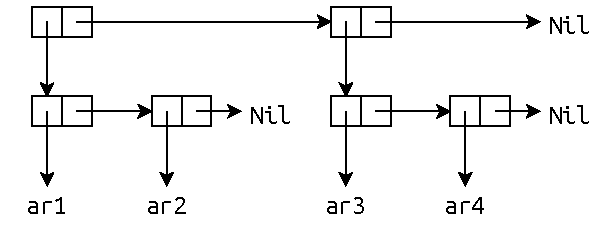
\includegraphics[scale=1]{img/1-7}
	\end{figure}

	\clearpage

	\item Написать функцию \texttt{(f ar1 ar2)}, возвращающую \texttt{((ar1) (ar2))}
	
\begin{lstlisting}[language=Lisp]
; lambda-выражение
(lambda (ar1 ar2)
	(list (cons ar1 Nil) (cons ar2 Nil))
)

; именованая функция
(defun f (ar1 ar2)
	(list (cons ar1 Nil) (cons ar2 Nil))
)
\end{lstlisting}

	\begin{figure}[ht]
		\centering
		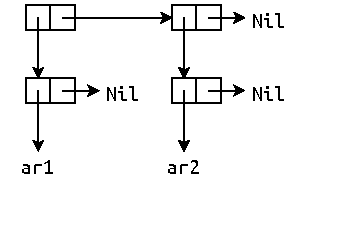
\includegraphics[scale=1.2]{img/1-8}
	\end{figure}
		
	\item Написать функцию \texttt{(f ar1)}, возвращающую \texttt{(((ar1)))}
	
\begin{lstlisting}[language=Lisp]
; lambda-выражение
(lambda (ar1)
	(cons (cons (cons ar1 Nil) Nil) Nil)
)

; именованая функция
(defun f (ar1)
	(cons (cons (cons ar1 Nil) Nil) Nil)
)
\end{lstlisting}

	\begin{figure}[ht]
		\centering
		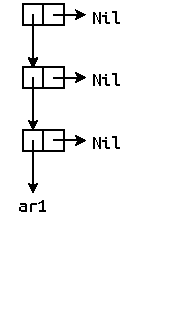
\includegraphics[scale=1.2]{img/1-9}
	\end{figure}

\end{itemize}
